\mychapter{3}{Opis riešenia - Server manažmentu rolí a používateľov}


%ked vyhladavam užívateľov, nemal by som dať limit... aj ked to mi neotestujú :D
\section{Určenie požiadaviek}
Aplikačným výstupom tejto bakalárskej práce je web stránka, ktorej účelom je vytvoriť jednoduché a intuitívne aplikačné rozhranie pre priraďovanie používateľov k rolám. 
Hlavné funkcionality zahŕňajú:

\begin{itemize}
	\item Zobrazenie všetkých používateľov vo firme
	\item Zobrazenie takých používateľov, ktorí nemajú vo firme priradenú rolu
	\item Zatriedenie používateľov podľa príslušnosti k rolám vo firme
	\item Utriedenie používateľov podľa rôznych kritérií - ID, meno, priezvisko, email
	\item Priradiť používateľov k role vo firme
	\item Odobrať používateľov z role vo firme
	\item Vytvoriť vo firme novú rolu
	\item Pridať do firmy role prostredníctvom XML súboru
	\item Odstrániť rolu z firmy -  pri odstránení roly z firmy, treba dať pozor, aby sme nemohli odstrániť také, ktoré firma práve používa na vykonávanie vlastných procesov
\end{itemize}

\noindent Zároveň má aplikácia poskytovať rozhranie k \emph{editoru rolí a organizačnej štruktúry} pre:
\begin{itemize}
	\item Načítanie rolí z firmy 
	\item Uloženie mapovania rolí ku Petriho sieti - uloženie rolí a referencií 
\end{itemize}







\section{Návrh}
%V tejto časti sa zameriame na podrobný opis implementácie modulu na správu a priraďovanie rolí k používateľom. Vysvetlíme fungovanie rolí v systéme, databázový model a popíšeme celkovú architektúru a spôsob implementácie rolí v našom systéme. Rozoberieme možné bezpečnostné riziká a spôsob ich riešenia. Navrhneme možné rozšírenia , ktoré vylepšia funkcionalitu a bezpečnosť.
%V tejto časti sa zameriame na podrobný opis implementácie modulu na správu a priraďovanie rolí k používateľom. Vysvetlíme fungovanie rolí v systéme, databázový model a popíšeme celkovú architektúru a spôsob implementácie rolí v našom systéme. Rozoberieme možné bezpečnostné riziká a spôsob ich riešenia. Navrhneme možné rozšírenia , ktoré vylepšia funkcionalitu a bezpečnosť.

\subsection{Popis architektúry} 
Základnou myšlienkou RBAC architektúry je odstrániť priame priraďovanie práv k používateľom. Tento výsledok sa zabezpečí pridaním medzikroku, a teda rolí medzi samotných používateľov a ich právomoci. Samotná implementácia RBAC značne závisí od konkrétneho systému. Naša aplikácia sa zameriava na vytvorenie WfMS za pomoci Petriho sietí. \\Ako prvé si definujeme základnú architektúru. Na obrázku \ref{fig:model_rbac_v_aplikacii} môžeme zreteľne vidieť dve nezávislé časti fungovania Workflow manažment systému. V ľavej časti ilustrácie vidíme sekciu, ktorá sa zaoberá  prideľovaním  používateľov k roliam, zatiaľ čo pravá časť znázorňuje proces samotný. Vo firme je vďaka tomu zabezpečené, aby sa procesy mohli vytvárať nezávisle od používateľov. Priraďovanie práv je zabezpečené väzbou medzi rolami a procesmi. Pre správnu funkcionalitu je však potrebné, aby firma mala priradené také roly, ktoré sú použité v jednotlivých procesoch, ktoré firma využíva. Definovanie prístupových práv je zabezpečené nad samotnými prechodmi v sieti.

\begin{figure}[h]
	\centering
	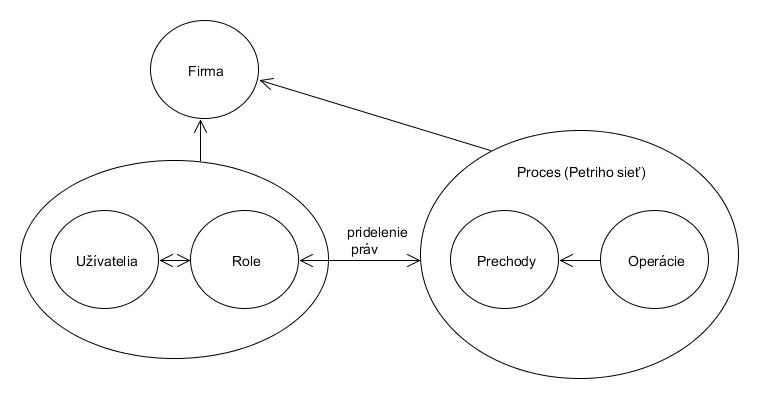
\includegraphics[width=0.9\linewidth]{images/roles_in_petri_model}
	\caption{ Model RBAC v aplikácii}
	\label{fig:model_rbac_v_aplikacii}
\end{figure}

\subsubsection{Priraďovanie používateľov k rolám}
V našej aplikácii nechceme, aby bol používateľ viazaný len na jednu firmu. Chceme, aby pod rovnakým účtom mohol figurovať vo viacerých firmách, prípadne mal možnosť si založiť vlastnú. Preto je potrebné, aby sa používatelia neviazali len na samotnú rolu. V aplikácii bude väzba používateľa na rolu závislá od konkrétnej firmy. V každej firme bude môcť administrátor - používateľ s právami na riadenie rolí, mať možnosť priradiť používateľa ku konkrétnej role, ktorá je vo firme zaradená. Samotný používateľ môže byť týmto spôsobom priradený vo viacerých firmách, pričom v každej firme bude mať iné práva.\\

 Na obrázku  \ref{fig:user_to_roles} môžeme vidieť zjednodušený model mapovania právomocí používateľa prostredníctvom systému rolí.
Šedé pozadie v roli znamená, že používateľ je k role priradený.  V rovnakom procese vidíme, že používateľ, ktorý môže vo firme 1 spustiť prechod 1 , nie je oprávnený vykonať prechod 1 aj vo firme 2, pretože v nej nemá priradenú rolu. Vo firme 2 môže spustiť iba prechod 2.

\begin{figure}[h]
	\centering
	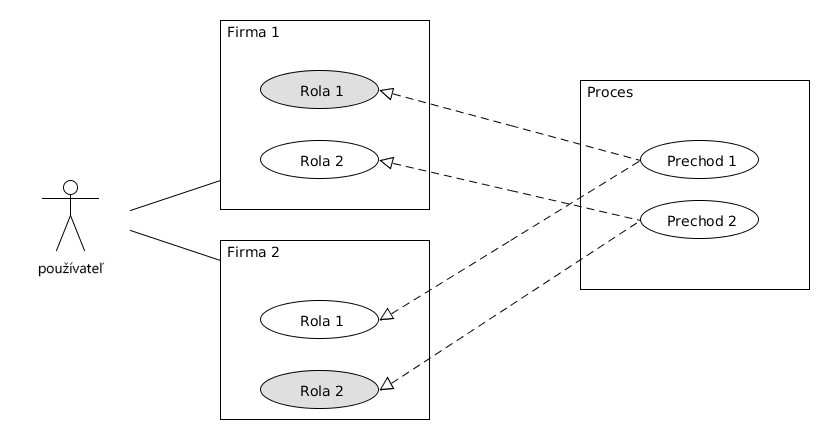
\includegraphics[width=0.9\linewidth]{images/user_to_roles}
	\caption{ Mapovanie používateľov na roly vo firme}
	\label{fig:user_to_roles}
\end{figure}


%\subsection{Riadenie právomocí}	
%Zadefinovali sme si ako sa v aplikácii mapujú používatelia na role. V nasledujúcej časti si bližšie definujeme pravidlá pre spúšťanie prechodov v sieti, rovnako ako aj samotné právomoci ktoré daná rola v procese nadobudne. 



\subsubsection{Priradenie práv k rolám}
Priradenie práv k rolám je definované nepriamo prostredníctvom jednotlivých prechodov. Hlavnou úlohou roly v procese je zadefinovať práva na vytváranie nových prípadov a takisto určiť právomoci na spúšťanie prechodov v procese. Schopnosť spustiť nový prechod je však vymedzená referenciami, návrhom Petriho siete a stavom, v akom sa tokeny momentálne nachádzajú.  


\begin{figure}[H]
	\centering
	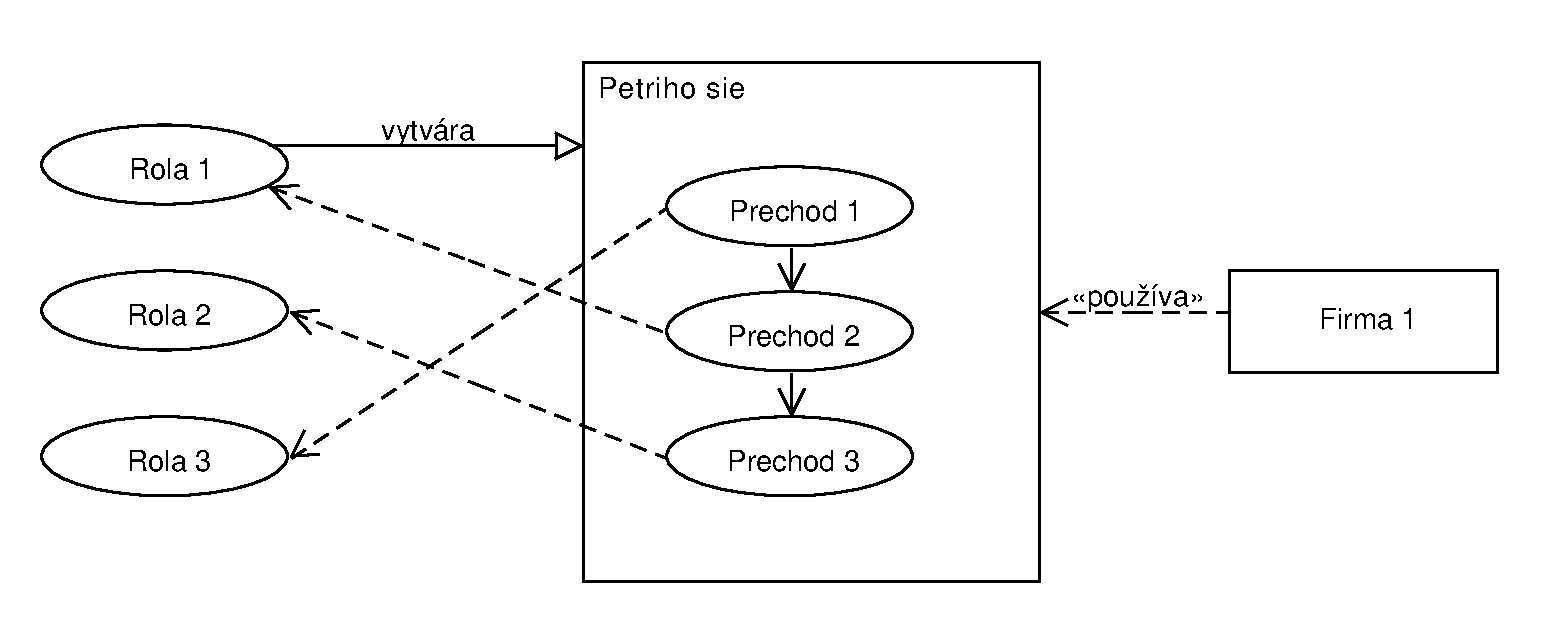
\includegraphics[width=0.9\linewidth]{images/roles_permissions}
	\caption{ Právomoci rolí v sieti }
	\label{fig:roles and permissions}
\end{figure}

\subsubsection{Definovanie prístupových práv ku prechodu}

Osoba môže v jednotlivom prípade spustiť prechod, ak spĺňa nasledovné požiadavky:
\begin{enumerate}
	\item prechod je spustiteľný
	\item osoba je priradená k role, ktorej prináleží daný prechod 
	\item osoba spĺňa požiadavky referencie
\end{enumerate}

Spustiteľnosť prechodu je zadefinovaná prostredníctvom Petriho siete. Prechod v sieti je spustiteľný len vtedy, ak každé  miesto vstupujúce do prechodu obsahuje minimálne toľko tokenov, aká je násobnosť hrany medzi daným miestom a prechodom.
V aplikácii máme dva typy referencií: \textbf{referenciu na prechod} a \textbf{referenciu na prvú rolu} .
Ak má prechod nastavenú \emph{referenciu na prechod}, v databáze sa porovná používateľove ID s používateľom , ktorý spustil referovaný prechod. V prípade, že tieto dáta súhlasia, používateľ je oprávnený spustiť prechod.

Ak má prechod nastavenú \emph{referenciu na prvého používateľa}, overí sa ,či sa v procese už daná rola nevyskytla. Ak prechod s danou rolou v danom prípade ešte nebol spustený, používateľ je oprávnený tento prechod spustiť. V opačnom prípade je potrebné overiť ID používateľa s používateľom, ktorý ako prvý spustil prechod s touto rolou. Ak sa zistí zhoda, používateľ môže daný prechod spustiť.



\subsubsection{Operácie nad prechodom}	
Práva, ktoré rola nad prechodom získa, sú zadefinované operáciami v konkrétnom prechode. Tieto operácie sa určia pri vytváraní formulára k danému prechodu (kapitola \ref{editor formulárov}).  
Vo formulári je možné nastaviť, aké dáta budú používateľovi prístupné, či ich bude môcť používateľ iba zobrazovať, alebo aj editovať. Takisto sa definuje, ktoré údaje je potrebné vyplniť, aby mohol používateľ tento prechod dokončiť.

\begin{figure}[H]
	\centering
	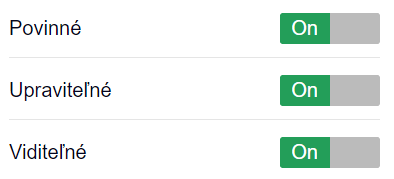
\includegraphics[width=0.4\linewidth]{images/formulare_opravnenia}
	\caption{ Právomoci definované v prechodoch }
	\label{fig:roles_permissions}
\end{figure}





\section{Implementácia}

\subsection{Modul na priraďovanie používateľov k rolám}
Vo WfMS treba zabezpečiť používateľsky ľahko zrozumiteľnú a jednoduchú administráciu rolí vo firme. Priraďovanie rolí vo firme je realizovaná na dvoch úrovniach: \emph{priradenie jednej roly pre viacero používateľov} a \emph{priradenie viacero rolí pre jedného používateľa}. Pre tieto účely sme vytvorili tabuľku, kde sa zobrazia jednotliví používatelia. Zoznam používateľov sa vytvorí na základe vybranej sekcie. Tieto sekcie delíme podľa filtra na \textbf{všeobecné} a \textbf{podľa rolí vo firme}. V prvej kategórii sú všetci používatelia a takí, ktorí nemajú priradenú rolu. V druhej zobrazujeme používateľov, ktorí sú priradení k určitej role. Používateľov je možné usporiadať v každej sekcii podľa ich ID, mena, priezviska alebo emailu. Zároveň je možné v každej sekcii na základe týchto kritérií vyhľadávať ľudí.

\begin{figure}[h]
	\centering
	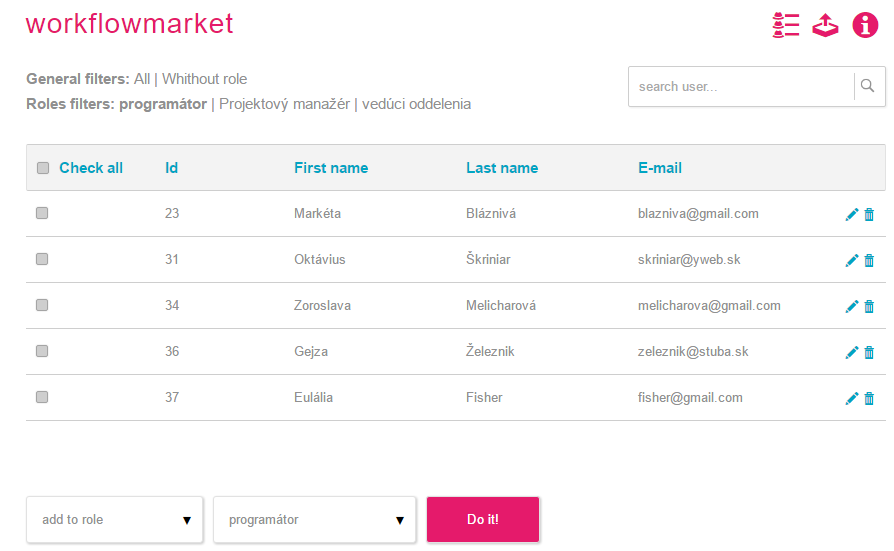
\includegraphics[width=0.9\linewidth]{images/server_roli_screen}
	\caption{ Prideľovanie používateľov k rolám }
	\label{fig:server_roli_screen}
\end{figure}

\subsubsection{Priradenie a vyradenie viacerých používateľov z role}
Priradenie a vyradenie viacerých používateľov je založené na dvoch krokoch. Označenie používateľov a následné vybranie žiadanej akcie - add to role (priradenie do role), delete from role (ich odstránenie z role).  

\begin{figure}[h]
	\centering
	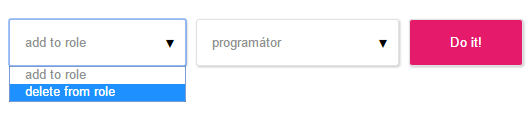
\includegraphics[width=0.5\linewidth]{images/role_actions_screen}
	\caption{ Výber akcie pre označených používateľov  }
	\label{fig:Výber akcie pre označených používateľov}
\end{figure}

\subsubsection{Priradenie a vyradenie jednotlivca}
Správa samotného používateľa je realizovaná viacerými spôsobmi. Prvý spôsob je rovnaký ako pri správe viacerých používateľov (označíme ale iba jedného používateľa). Druhý spôsob je detailná správa používateľa. Po kliknutí na podrobnosti konkrétneho používateľa sa zobrazí okno pre konkrétneho používateľa. V ňom sú všetky roly, do ktorých je možné používateľa priradiť. Jednoduchým kliknutím na tlačítko sa používateľ priradí alebo odstráni z role. Takisto je možné odstrániť používateľa z roly priamo z tabuľky kliknutím na ikonu smetného koša.

\begin{figure}[h]
	\centering
	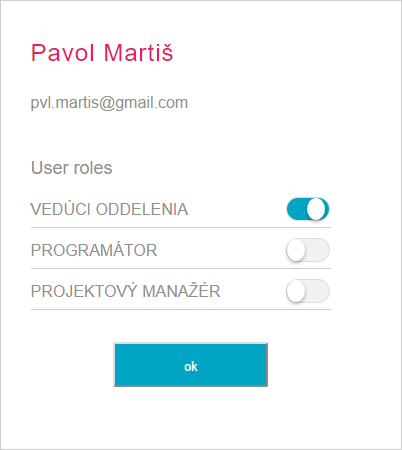
\includegraphics[width=0.5\linewidth]{images/user_detail_screen}
	\caption{ Správa rolí pre konkrétneho používateľa  }
	\label{fig:user_detail_screen}
\end{figure}

\begin{figure}[h]
	\centering
	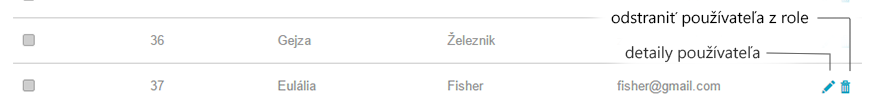
\includegraphics[width=1\linewidth]{images/one_user_screen2}
	\caption{Možnosti pre konkrétneho používateľa priamo z tabuľky  }
	\label{fig:user_table}
\end{figure}

\subsubsection{Správa rolí vo firme}
Firma musí mať vo svojej štruktúre také roly, ktoré používa vo svojich procesoch. Preto sa pri priradení procesu do firmy nahrávajú do firmy roly, ktoré sú v procese využívané. Okrem toho sa však dajú vo firme vytvoriť roly pred tým, ako sa k nemu priradia procesy. Na to slúži administrácia rolí vo firme. Do firmy je tak možné pridať nové roly, prípadne odstrániť staré. Pri odstraňovaní rolí sa najprv skontrolujú v databáze, či firma nepoužíva danú rolu v niektorej z jej procesov.

\begin{figure}[h]
	\centering
	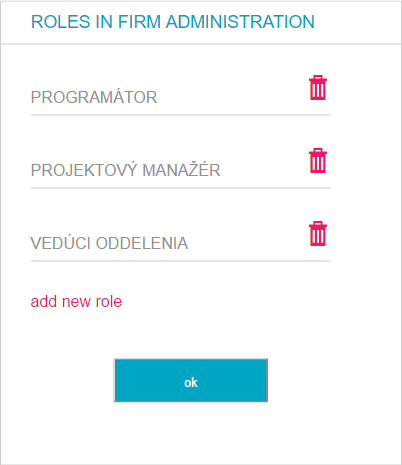
\includegraphics[width=0.5\linewidth]{images/firm_administration_screen}
	\caption{ Administrácia rolí vo firme  }
	\label{fig:Administrácia rolí vo firme}
\end{figure}

\noindent Priradenie rolí do firmy je možné aj za pomoci XML súboru v podobnej štruktúre:
\begin{lstlisting}[language=XML]
<?xml version="1.0" encoding="UTF-8"?>
<document>
	<roles>
		<role>
			<name>názov role 1</name>
		</role>
		<role>
			<name>názov role 2</name>
		</role>
	</roles>
</document>
\end{lstlisting}


\subsection{Ukladanie rolí a referencií z editoru do databázy}
\label{ukladanie rolí}
Dôležitou časťou serverovej časti rolí je uložiť výstup z \emph{editora rolí}. Celý proces prebieha v nasledovných fázach : 
\begin{enumerate}
	\item Vytvorenie a priradenie rolí (v editore)
	\item Následne po tom, ako používateľ odošle požiadavku na uloženie do databázy,  sa odošle na server XML súbor spolu s ID procesom  a ID firmy z databázy
	\item Na serveri sa najprv vymažú staré dáta (napojenie rolí a referencií na sieť), aby nevznikali problémy pri spätnej úprave
	\item Do databázy sa pridajú roly
	\item Do databázy sa pridajú spojenia medzi rolou a prechodmi. Uloží sa rola, ktorá môže spustiť prípad a pridajú sa referencie ku prechodom.
	\item Roly použité v sieti sa priradia do firmy v ktorej sa vykonávalo modelovanie
\end{enumerate}

Príklad XML súboru pre uloženie do databázy:

%\<\!\-\-  \-\-\>
%referencia na prvého používateľa z roly
%<!-- referencia na prechod s id 0 -->
\begin{lstlisting}
<?xml version="1.0" encoding="UTF-8"?>
<document>
<roles>
	<role>  // definovanie role 
		<id>0</id>
		<name>programátor</name>
		<start_case>false</start_case> // určuje či môže rola spustiť prechod
		<transitionId>0</transitionId> 
		<transitionId>1</transitionId>
		<transitionId>2</transitionId>
	</role>
</roles>
<references>
	<reference> // nulová referencia 
		<transitionId>2</transitionId>
		<value>false</value>
	</reference>
	<reference>   // referencia na prechod s id 0
		<transitionId>1</transitionId>
		<value>true</value>
	</reference>
		<reference> 
		<transitionId>0</transitionId>
		<value>0</value>
	</reference>
</references>
</document>
\end{lstlisting}


\subsection{Dátový model}
Dátová časť našej aplikácie je implementovaná v databáze MySQL. Na začiatku je potrebné definovať návrh tabuliek pre uloženie rolí a referencii ku konkrétnej sieti (obr. \ref{fig:Priradenie právomocí rolám}). 

\begin{figure}[h]
	\centering
	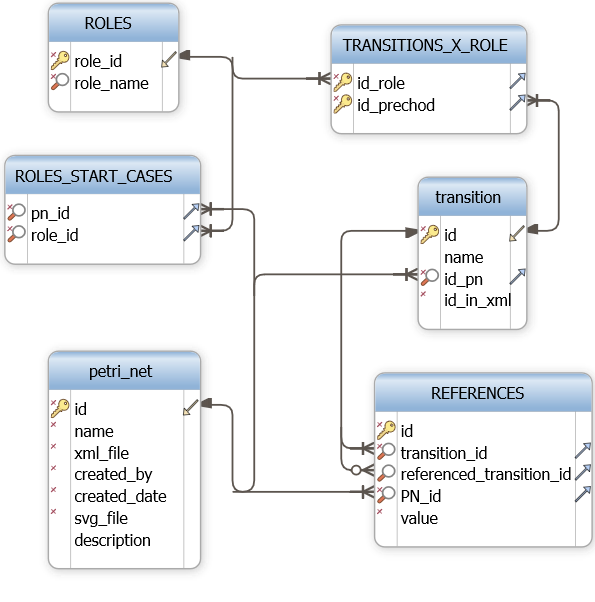
\includegraphics[width=0.7\linewidth]{images/roles_permissions_diagram}
	\caption{ Priradenie právomocí rolám }
	\label{fig:Priradenie právomocí rolám}
\end{figure}
Do tabuľky ROLES budeme ukladať role a ich názov. Táto tabuľka má okrem ID ako unikátny atribút takisto \emph{názov roly}. Tabuľka \emph{TRANSITIONS\_X\_ROLE} ukladá právomoci rolí na spustenie konkrétneho prechodu v sieti, tabuľka \emph{ROLES\_START\_CASES}  ukladá rolu, ktorá môže spustiť nový prípad a tabuľka REFERENCES ukladá jednotlivé referencie ku prechodom. Ak má nastavené \emph{value} na false, prechod nemá referenciu. Ak má hodnotu nastavenú na true , skontroluje sa položka \emph{referenced\_transition\_id}. Pokiaľ má tento atribút číselnú hodnotu, referencia odkazuje na prechod s touto ID. Pokiaľ má nastavenú hodnotu na NULL, referencia je nastavená na prvého užívateľa z role.



Druhým krokom je návrh databázového modelu, ktorý bude umožňovať konkrétnym používateľom vo firme priradiť rolu (obrázok \ref{fig:Priradenie používateľov do rol vo firmách}). Priradených používateľov vo firme zaznamenávame v tabuľke USERS\_X\_FIRM. Ich priradenie k rolám vo firme je uložené v tabuľke USERS\_X\_ROLES. Priradenie rolí do firmy je zabezpečené takisto priamo prostredníctvom tabuľky ROLES\_X\_FIRM.
\begin{figure}[H]
	\centering
	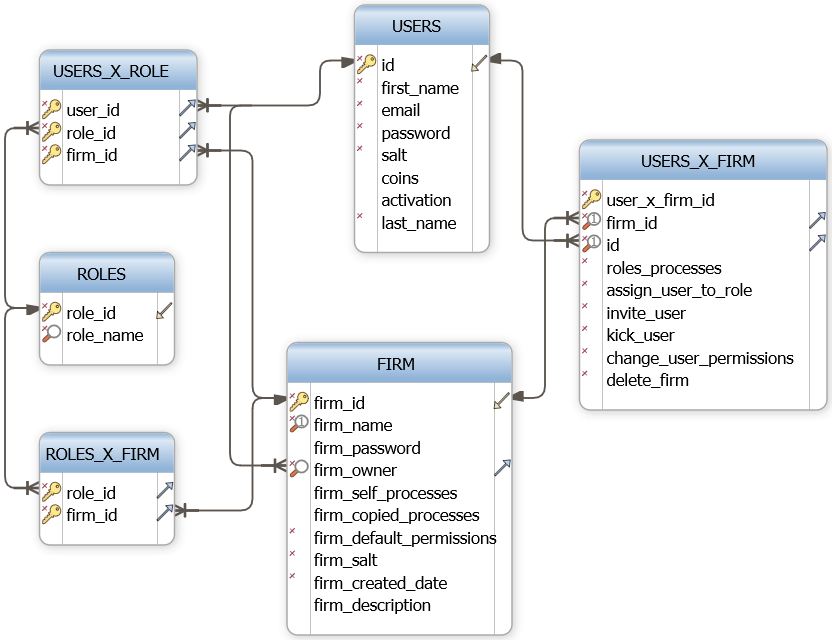
\includegraphics[width=1\linewidth]{images/users_to_roles_diagram}
	\caption{ Priradenie používateľov do rol vo firmách }
	\label{fig:Priradenie používateľov do rol vo firmách}
\end{figure}



%Vyrieši sa tak aj ukladanie roly do databázy. Zo samotného XML súboru sa nedá zistiť, či už neexistuje v databáze rovnaká rola priradená k prechodu inak ako podľa názvu roly. \\

Nakoniec na obrázku \ref{fig:tabulky_pre_role} môžeme vidieť spojenú  relačnú databázu pre potreby serverovej časti rolí.

\begin{figure}[H]
	\centering
	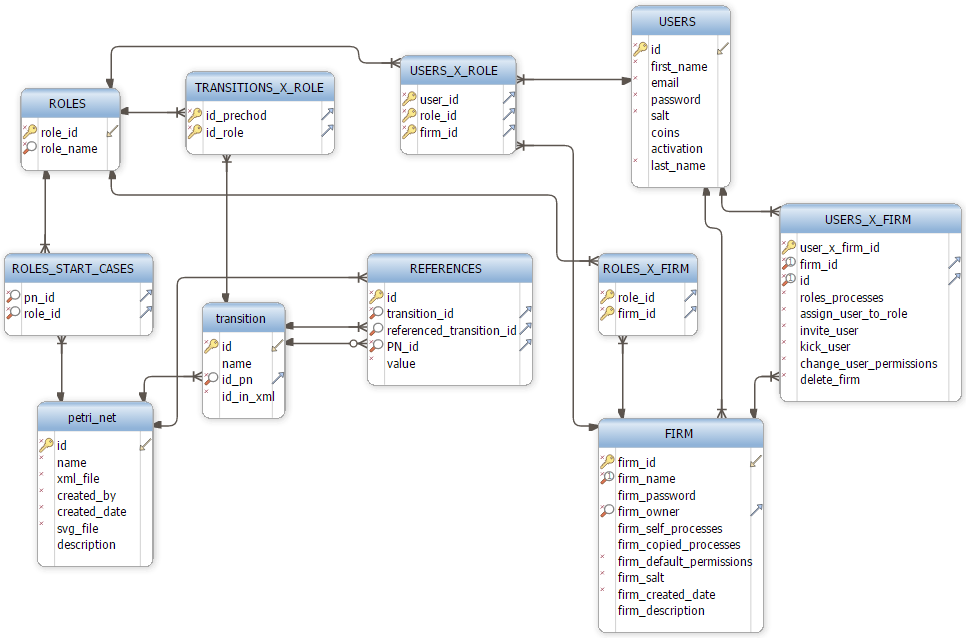
\includegraphics[width=1\linewidth]{images/database_diagram}
	\caption{ Hlavné tabuľky pre prácu s rolami }
	\label{fig:tabulky_pre_role}
\end{figure}




\section{Testovanie riešenia}
\subsection{Používateľská skúsenosť}
V testoch pre používateľskú skúsenosť na \cite{attensee} dopadla stránka nadpriemerne dobre. Testovali sme záujmové body webovej stránky na vzorke 38 účastníkov. Z testov (obrázok \ref{fig: Hlavné záujmové body používateľa} , \ref{fig:Mapa pozornosti}) sme zistili, že hlavné elementy na stránke boli pre používateľov dostupné a zrozumiteľné.  
Všimli sme si však, že administrácia konkrétneho používateľa a stránkovanie nebolo dobre viditeľné. 

\begin{figure}[H]
	\centering
	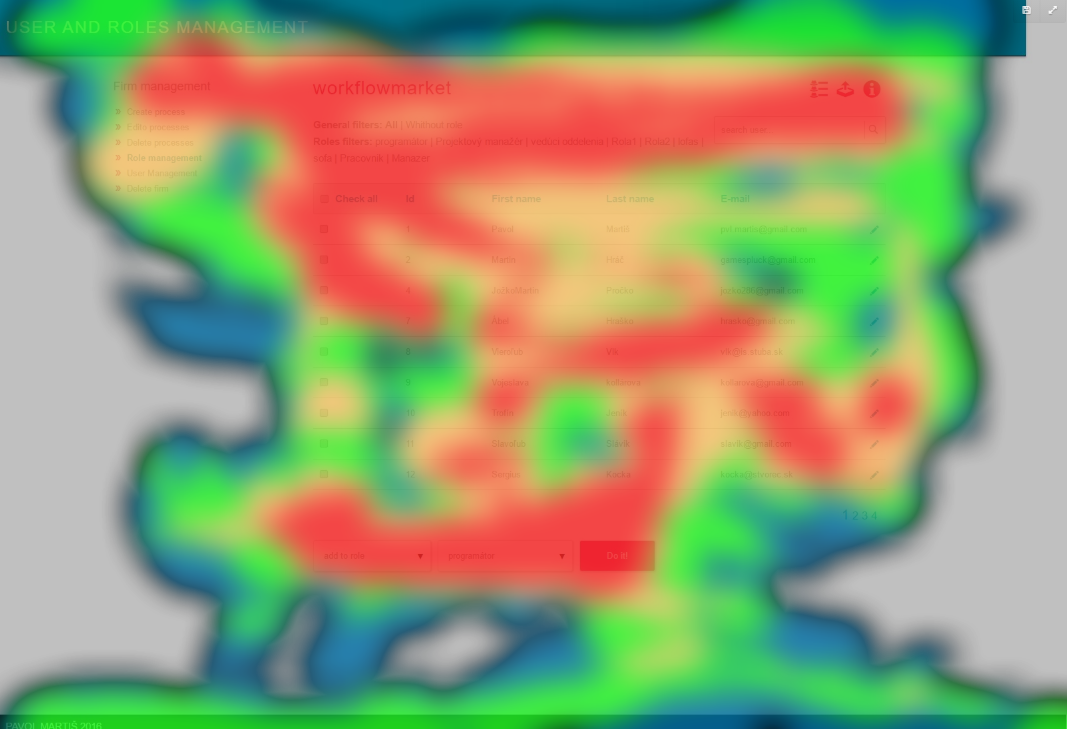
\includegraphics[width=0.7\linewidth]{images/heatmap}
	\caption{Mapa zobrazujúca hlavné body pozornosti používateľa}
	\label{fig:Mapa pozornosti}
\end{figure}

\begin{figure}[H]
	\centering
	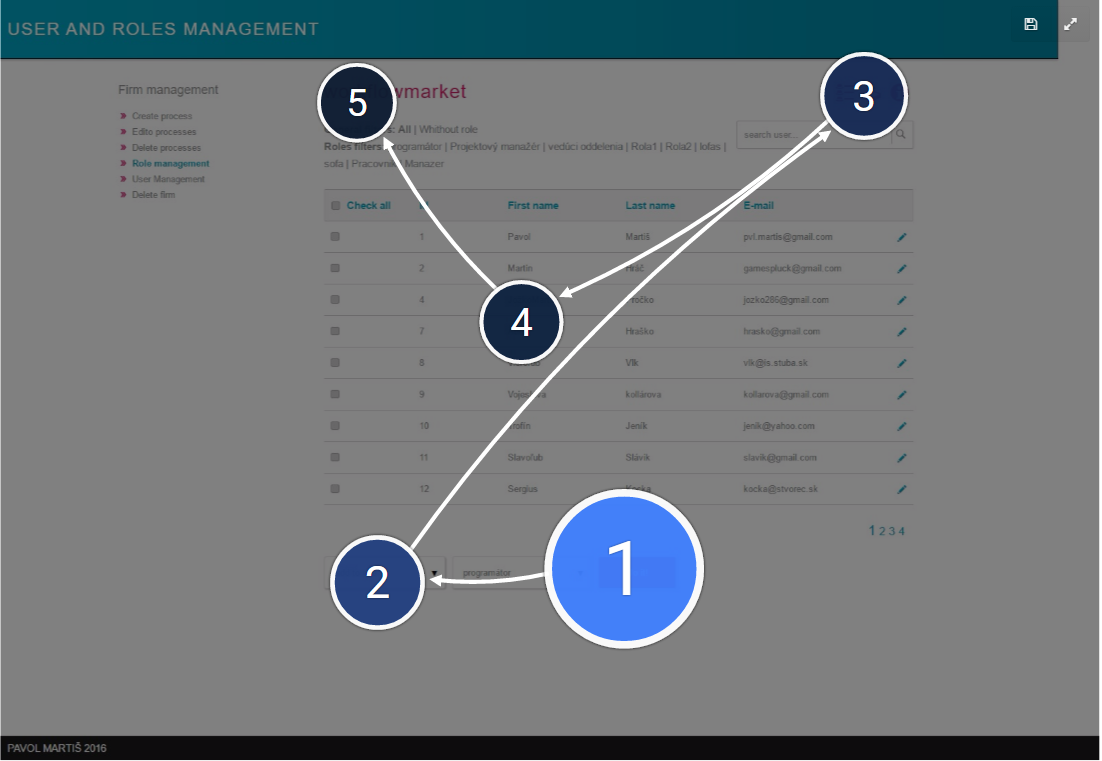
\includegraphics[width=0.7\linewidth]{images/path}
	\caption{ Hlavné záujmové body používateľa }
	\label{fig: Hlavné záujmové body používateľa}
\end{figure}




\subsection{Google testovanie}
Stránka dosiahla na Google PageSpeed Tool \cite{page_speed} dobré výsledky pre rýchlosť na počítači. Hlavné možnosti vylepšenia sa ponúkajú kompresia súborov a ukladanie do vyrovnávacej pamäti. Stránka však má nedostatky pre mobilnú verziu, pretože nespĺňa základné požiadavky na responzívny dizajn. 



\begin{figure}[H]
	\centering
	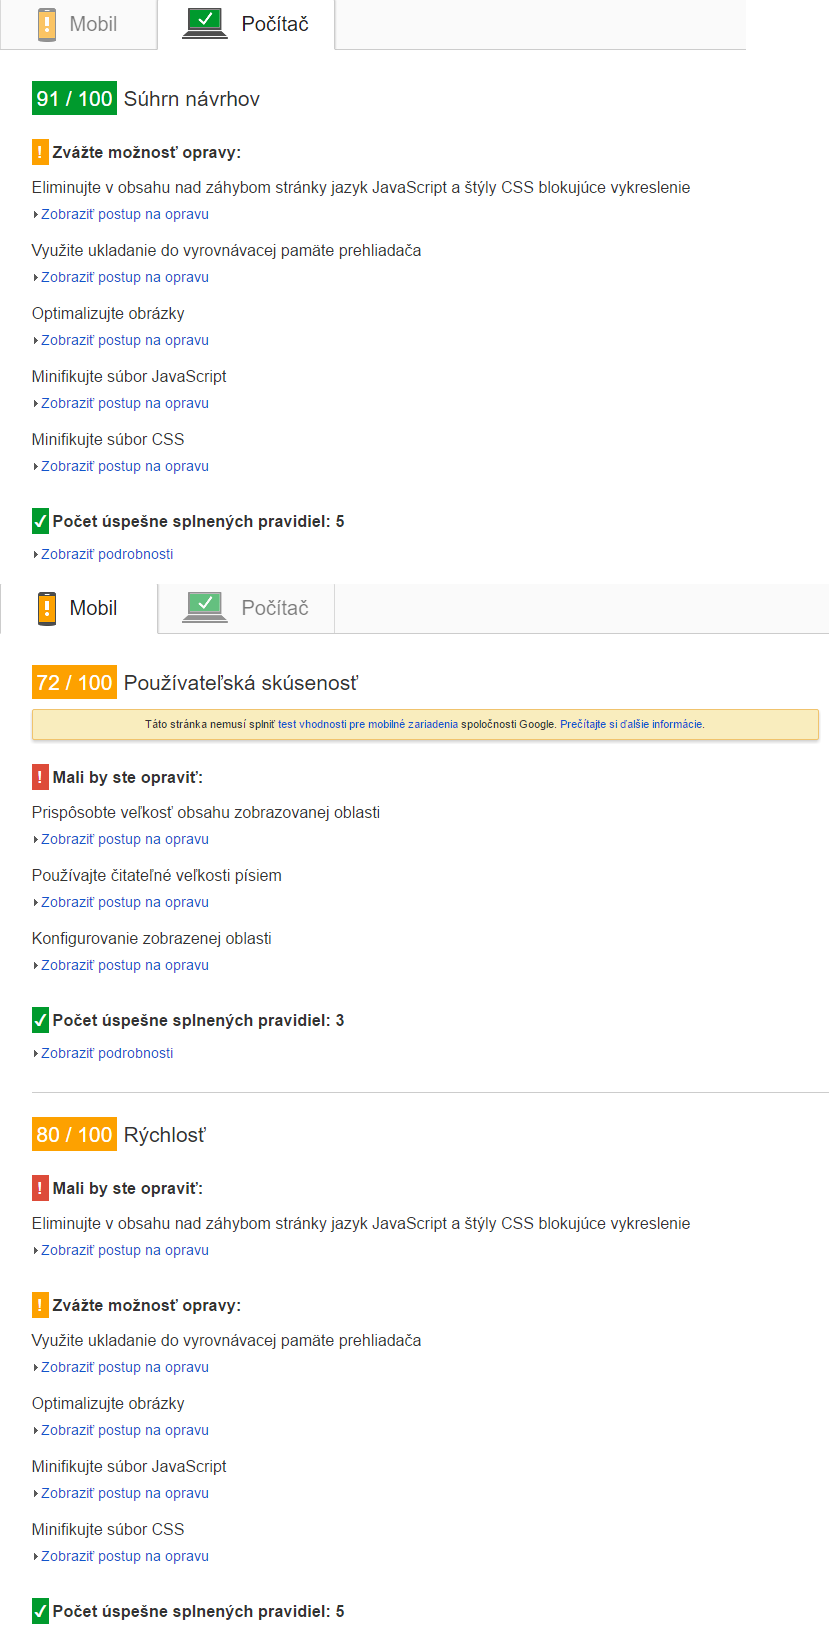
\includegraphics[width=0.7\linewidth]{images/mobil}
	\caption{ Výsledky rýchlosti pre mobil }
	\label{fig:Výsledky rýchlosti pre mobil}
\end{figure}

\subsection{Bezpečnosť}
Zistili sme nedostatky v bezpečnosti. Osoba, ktorá môže priraďovať a upravovať role vo firme môže jednoduchou zmenou html kódu alebo javascript súboru prepísať dôležité premenné a zasiahnuť do databázy inej firmy. V budúcnosti preto bude potrebné overovať právomoci administrátora pri jednotlivých prístupoch a zmenách v databáze. 

\subsection{Možné rozšírenia}
Ako hlavné rozšírenia sa ponúkajú dve dôležité časti. Doimplementovať hierarchiu rolí a pridať obmedzenia na kvalitatívnejšie oddelenie právomocí.
\\

Hierarchia rolí by mala umožňovať jasne definovať štruktúru rolí, tak, aby verne odzrkadľovala štruktúru v organizácii. Určia sa nadradené a podradené roly. Nadradené roly budú automaticky dediť právomoci podradených rolí. Zjednoduší sa tým organizácia štruktúry v podniku. V aktuálnej verzii aplikácie je potrebné používateľa prideliť do každej roly osobitne. Prípadným riešením bude vytvoriť v databáze novú tabuľku, kde budú priradené vzťahy medzi jednotlivými rolami v konkrétnej firme. K tomu bude treba vytvoriť nástroj na definovanie organizačnej štruktúry a zároveň bude potrebné predefinovať procesnú logiku systému. 

Ako súčasť tohto rozšírenia bude možnosť zjednotiť vo firme viacero rolí do jednej. V aktuálnej verzii vzniká problém pri priradení procesu do firmy, pretože firma musí automaticky prebrať všetky role v procese. Môže však nastať situácia, keď bude vo firme veľa rolí s rovnakou funkcionalitou, ale odlišným názvom. Ako príklad si môžeme zobrať rôzne synonymá. Rola programátor sa dá nazvať ako  ''programátor'', ''vývojár'', ''developer'' a takisto problém môžu spôsobovať viacjazyčné preklady.\\

Ďalším rozšírením bude pridanie obmedzení právomocí pre jedného používateľa. Pri modelovaní návrhu rolí v editore (kap. \ref{Editor manažmentu rolí a organizačnej štruktúry}) chceme pridať ku prechodu možnosť zápornej referencie. To bude znamenať, že jeden používateľ nebude môcť spustiť dva prechody,  ktoré sa vylučujú. Znamená to teda, že pokiaľ používateľ spustí prvý prechod, nebude schopný vykonať aj druhý prechod, ak obsahuje zápornú referenciu na prvý prechod. Za zváženie taktiež stojí obmedzenie štruktúry rolí pomocou statického vylúčenia práv. Znamenalo by to, že budú existovať určité obmedzenia pri priraďovaní používateľov k rolám. Administrátor by teda nebol schopný priradiť jednému používateľovi dve navzájom sa vylučujúce role.

Tretie rozšírenie by mohlo definovať štruktúru zamestnancov vo firme z hľadiska ich organizačnej a geografickej odlišnosti. Väčšie firmy majú viacero oddelení, ktoré môžu znázorňovať isté pracovné alebo geografické odlišnosti. Príkladom môžu byť rôzne oddelenia, ktoré v rámci firmy pracujú na odlišných objednávkach (respektíve prípadoch). V našom systéme by sa takto mali dať priradiť isté organizačné jednotky pri samotnom vytváraní nového prípadu, prípadne inak ošetriť, aby sa zamedzil prístup v rámci jednotlivých oddelení.



